\chapter{Религиозный римский гамбит}



%Зачем римлянам понадобилось христианство, и как оно спасло Европу от уничтожения.


История о том, как римляне спасли угольки цивилизации предвидя своё крушение, чтоб потом ветры истории раздули их в великие европейские империи, над которыми никогда не заходит солнце. Накидывал тезисно, уместился в десять пунктов с послесловием, и текст закончен сам по себе. Но каждый из пунктов можно дополнительно разворачивать в комментариях, они для этого даж пронумерованы специально. Ну и автор не стремится оскорбить чьи-то религиозные чувства, и рассматривает христианство в чисто историческом контексте, не более того.



\begin{figure}[h!tb]
	\centering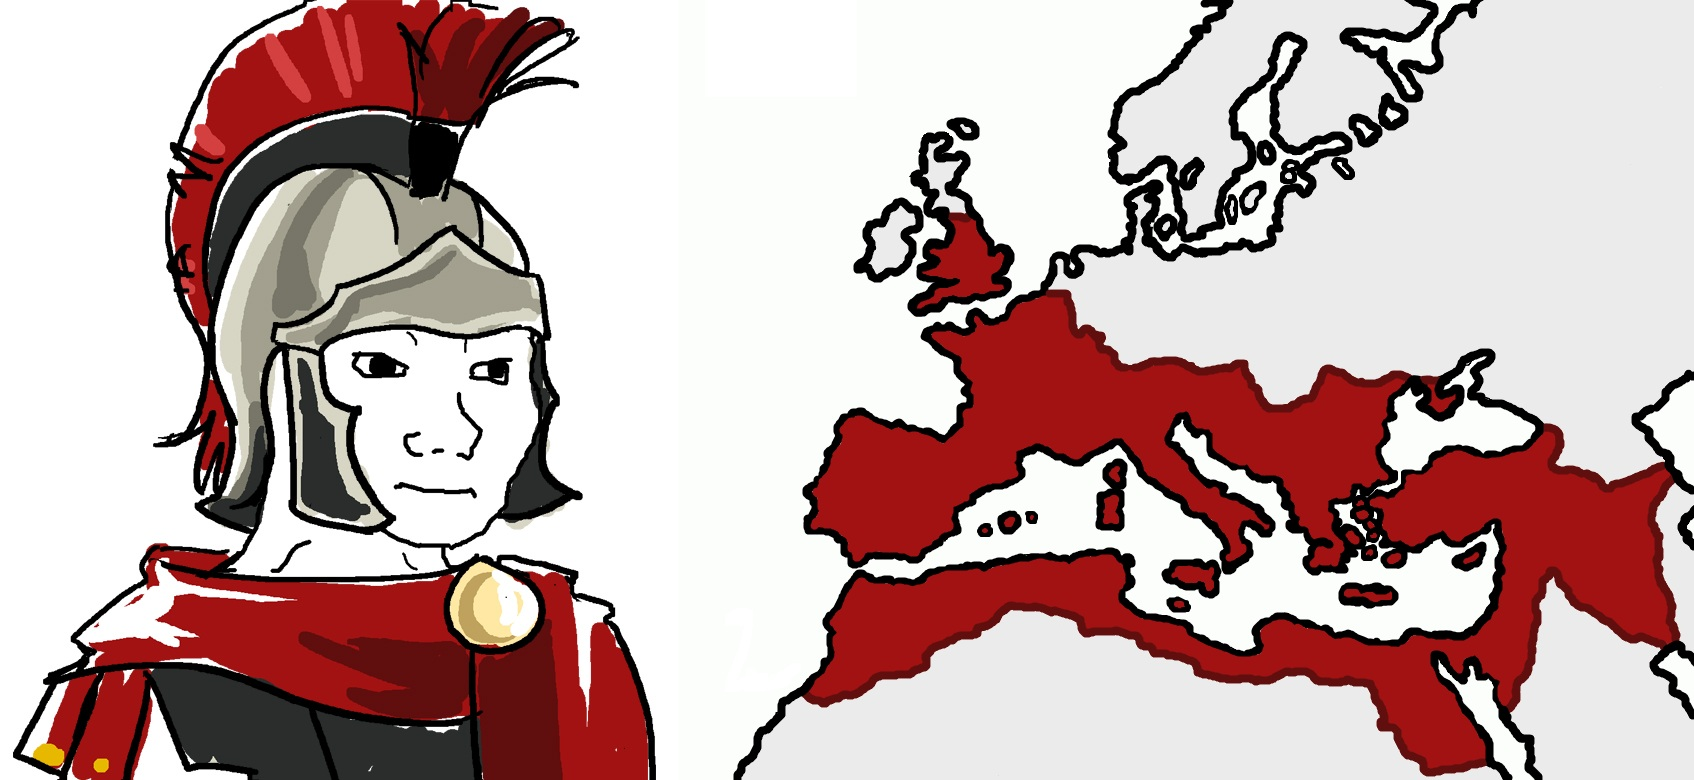
\includegraphics[scale=0.3]{Relig_gambit/1572931902173172101.png}
	\caption{Максимальные границы, при Траяне (117г н.э.). Дальше, как говорится, было только хуже.		}
	\label{fig:gambit1} % Unique label used for referencing the figure in-text
	%\addcontentsline{toc}{figure}{Figure \ref{fig:placeholder}} % Uncomment to add the figure to the table of contents
	
\end{figure}

\section{Отношение римлян к религии как таковой}

Несмотря на христианские байки про жуткие религиозные гонения, в плане религии в Ранней Империи с этим делом всё было более чем толерантно. Культов было дохрена и больше, как официальных (весь римский пантеон), так и локальных божков всех народов имперки, тысячи их. Римляне никогда напрямую не лезли в вопросы веры своих граждан. Долбили конкретных христиан, за конкретные косяки, а именно за отрицание римского порядочка и откровенную сектантность. Любимым приёмом тогдашних христиан было обращать в свою веру римскую молодёжь (наследников крупных состояний, как правило) или уже наполовину впавших в маразм престарелых патрициев. Естественно, с отжиманием в пользу религиозной общины всего их имущества. Отчего другие римляне, видя как капиталы уходят каким-то тамошним свидетелям иеговы - горели жопой и требовали чтобы этих жуликов скармливали львам, по возможности. Имперская машина же бесилась от того, что эти христиане налогов не платят, не работают, хуйней какой-то занимаются и всячески кладут залупу на органы местного управления. За это, собственно, их и гоняли, но без какого-то религиозного экстаза. Это было общество, де-факто, атеистов, которые боролись с религиозным мракобесием, мешающим гражданскому обществу существовать. И очень по лайту. Христианство - игрушка знати, городская религия прежде всего. Напоследок посмотрите на то как римляне решали религиозные вопросы, если их конкретно заебать - Иудея. Там просто всех кого могли перехуярили, все что связано с религией - разрушили, а оставшихся выселили за черту оседлости. Римляне умели решать такие вопросы, но тут прост пинали в фоновом режиме и за конкретные косяки, по местному уголовному кодексу.



\begin{figure}[h!tb]
	\centering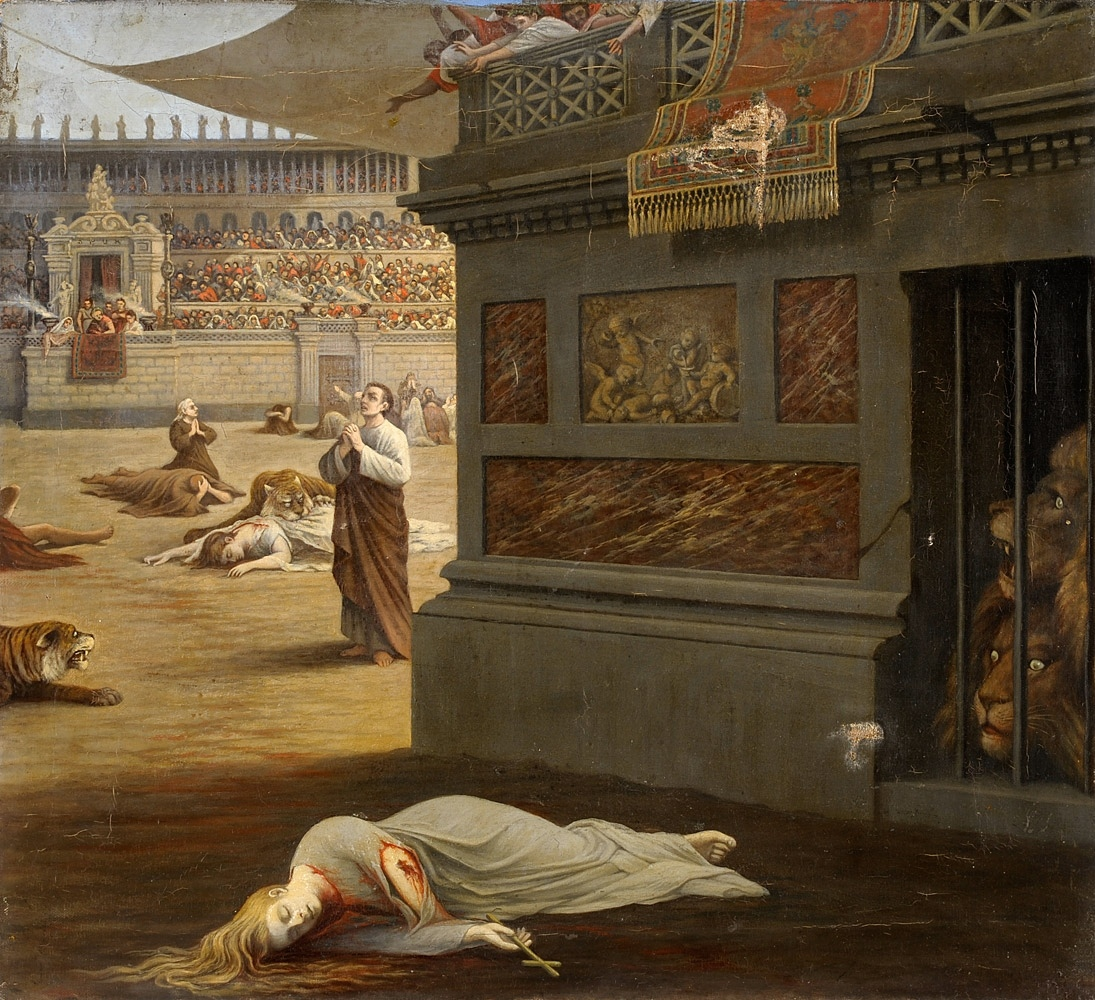
\includegraphics[scale=0.35]{Relig_gambit/15729320001204595.png}
	
	%	\caption{Небольшая подборка на тему любимого религиозного сюжета — «Львы едят христиан». Очень смешные картинки, особенно обратите внимание на львиные морды.		}
	\caption{Пример творчества  на тему любимого религиозного сюжета — «Львы едят христиан».}
	\label{fig:gambit21} % Unique label used for referencing the figure in-text
	%\addcontentsline{toc}{figure}{Figure \ref{fig:placeholder}} % Uncomment to add the figure to the table of contents
	
\end{figure}
%\begin{figure}[h!tb]
%	\centering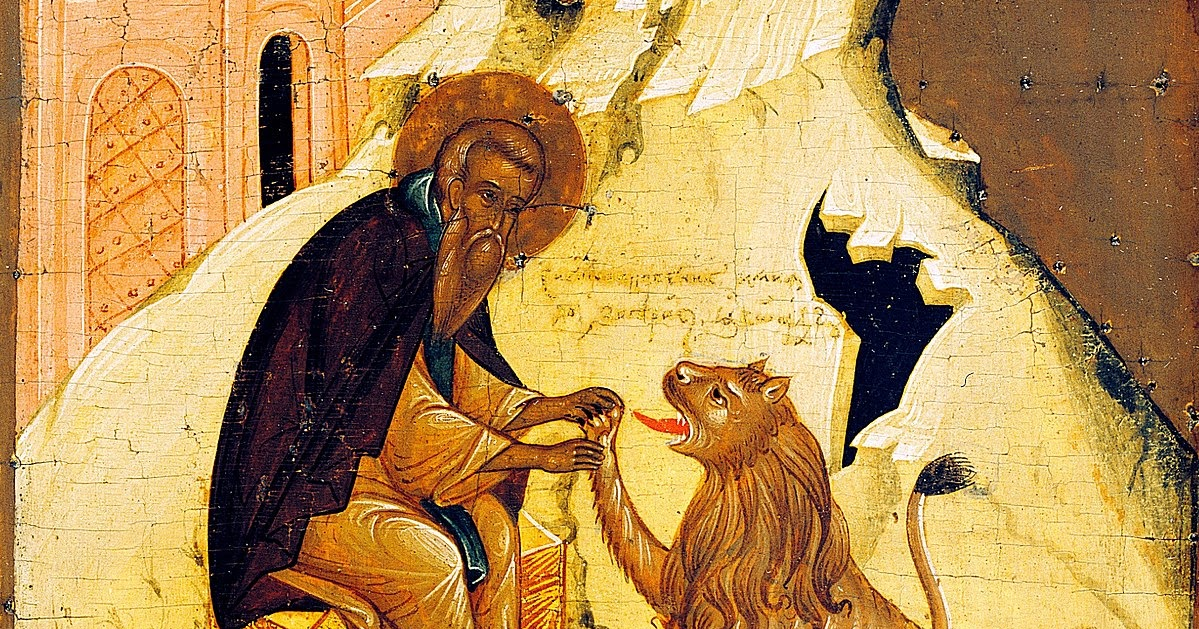
\includegraphics[scale=0.3]{Relig_gambit/157293206417861157.png}
%	\label{fig:gambit22} % Unique label used for referencing the figure in-text
%	%\addcontentsline{toc}{figure}{Figure \ref{fig:placeholder}} % Uncomment to add the figure to the table of contents
%	
%\end{figure}
%\begin{figure}[h!tb]
%
%	\centering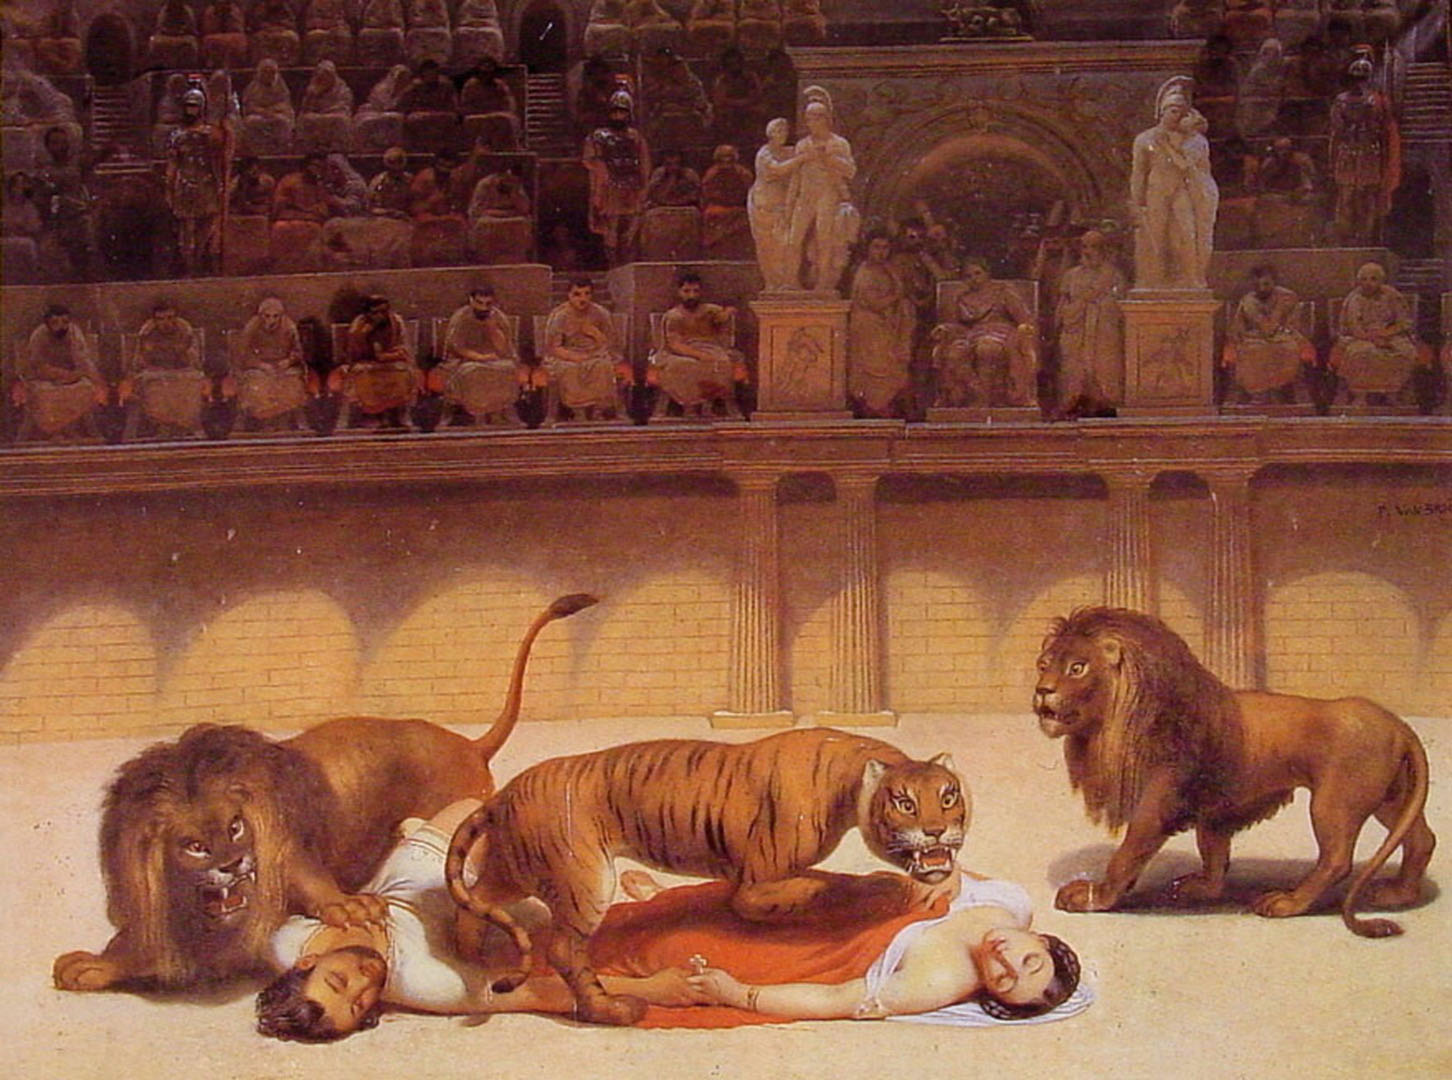
\includegraphics[scale=0.3]{Relig_gambit/1572931964163533241.png} 
%	\label{fig:gambit23} % Unique label used for referencing the figure in-text
%	%\addcontentsline{toc}{figure}{Figure \ref{fig:placeholder}} % Uncomment to add the figure to the table of contents
%	
%\end{figure}
%\begin{figure}[h!tb]
%	\centering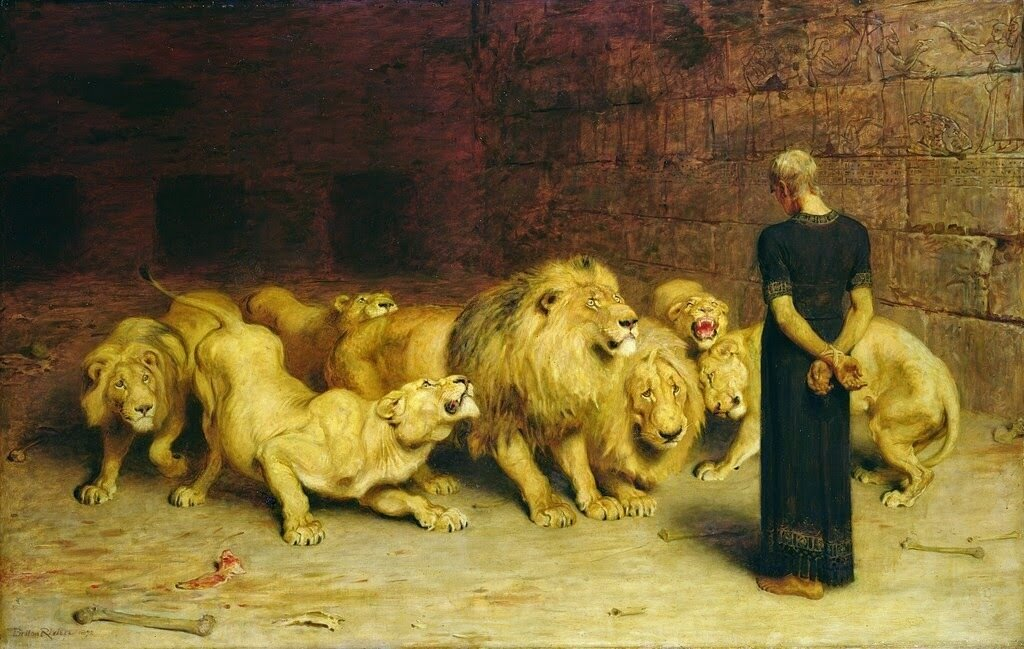
\includegraphics[scale=0.3]{Relig_gambit/1572931991162448764.png} 
%	\label{fig:gambit24} % Unique label used for referencing the figure in-text
%	%\addcontentsline{toc}{figure}{Figure \ref{fig:placeholder}} % Uncomment to add the figure to the table of contents
%	
%\end{figure}
%\begin{figure}[h!tb]
%	\centering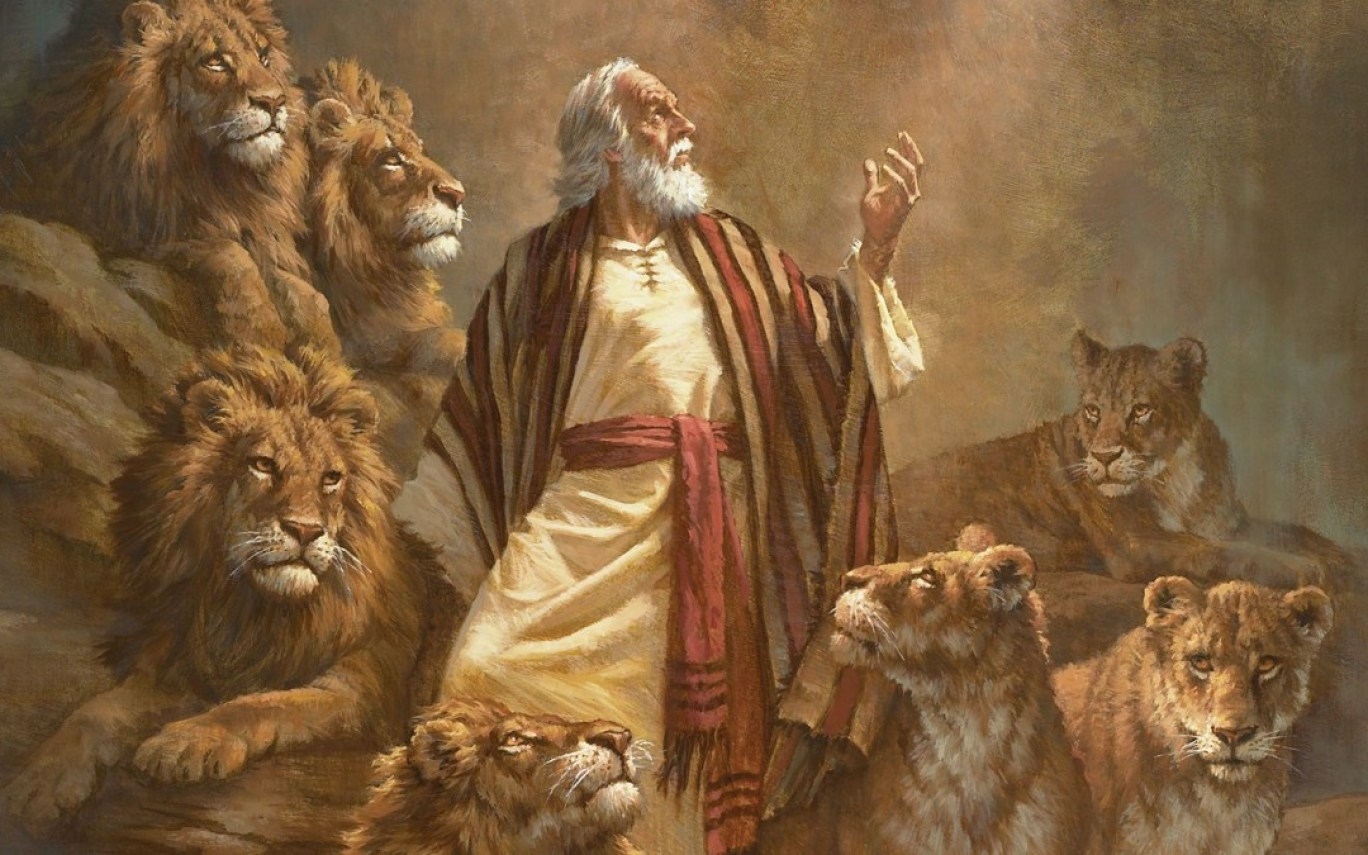
\includegraphics[scale=0.2]{Relig_gambit/1572932052172990351.png}
%	\label{fig:gambit25} % Unique label used for referencing the figure in-text
%	%\addcontentsline{toc}{figure}{Figure \ref{fig:placeholder}} % Uncomment to add the figure to the table of contents
%	
%\end{figure}
\section{Кризис Третьего Века (211-284г н.э)}
\begin{figure}[h!tb]
	\centering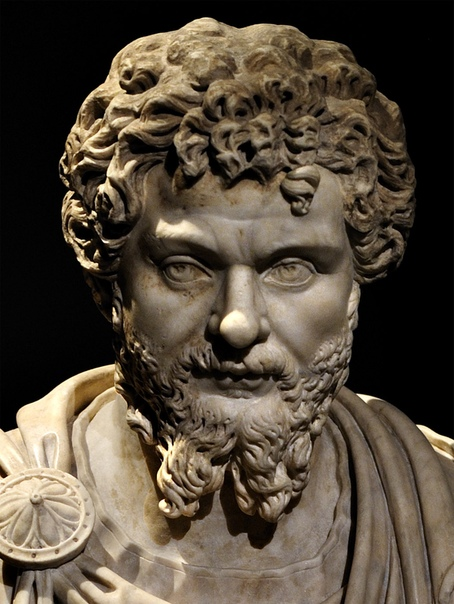
\includegraphics[scale=0.5]{Relig_gambit/157293210416964768.png}
	\label{fig:gambit3} % Unique label used for referencing the figure in-text
	%\addcontentsline{toc}{figure}{Figure \ref{fig:placeholder}} % Uncomment to add the figure to the table of contents
	\caption{Септимий Север собственной персоной, с лицом лягухи смотрит как его потомки катят имперку в Адъ и Израиль. 	}
\end{figure}

Если не вдаваться в детали, то за следующие десятилетия (211-284г н.э) сменилось штук двадцать императоров, произошло полсотни только крупных восстаний, бунтов и переворотов, армия бунтовала наравне со всеми остальными, границы рухнули и в имперку ломанулись варвары, экономика перестала существовать и вообще творился полный пиздец. Когда нибудь я про эту чехарду напишу отдельно, пока просто поверьте — это была клиническая смерть Римской Империи как явления, потом её пришлось, фактически собирать заново, и прежней она уже не была никогда.


Потом, после Септимия Севера, имперка начала трещать по швам и откровенно разваливаться. Римское самосознание, с помощью которого они пенетрировали всю Европу, потихоньку выветрилось, и после череды страшных гражданских войн было принято решение посадить это всё на клей. Концепция "один народ, один язык, одна вера, один фюрер" в действии. Именно тогда, кстати, всех жителей Имперки окончательно уравняли в правах, например. Но нам тут интересно другое. На месте идеологии и, яб даже сказал, идентичности, зияла здоровенная дыра, надо было чем-то её заполнить. И светское общество тут предложить не могло ничего, до времен национал-социализма, коммунизма и прочих "измов" ещё без малого две тысячи лет. А в религиозной жизни, как видно из пункта 1, творился полный пиздец. Локальные культы, каждый дрочит как хочет и молится чему угодно. Вот тут и пригодилось это наше христианство.

\section{ Религиозная реформа Константина (313-337г н.э.)}

Оно, христианство, было всё ещё подпольным и гоняемым, но уже достаточно мощным культом. Со временем из жуликоватых ранних христиан они превратились в респектабельных проповедников, "ушли в народ", и, в силу этого, растеряли большую часть радикального анархизма, потеряли ближневосточную специфику и перестали прыгать на светскую власть имперской бюрократии. И тут, при Диоклетиане (303г н.э.), их начали последний раз мощно гонять, лет десять старательно выкорчевывая по всей имперке, тратя кучу сил и ресурсов. Что особого успеха не имело, христиане заимели себе кучу всяких мучеников и организованно ушли в подполье. Римляне поняли что это не работает, подумали и зашли с другой стороны. "Не можешь помешать - возглавь". Внезапно в имперке при Константине мутится религиозная реформа, христианство получает статус государственной религии, лично император со всем семейством и большей частью знати одномоментно становятся ярыми христианами, а церковь органично включается в имперскую машину управления. После чего, естественно, начинается системная зачистка всех остальных религиозных культов. Ещё раз, до принятие христианства там творился полный плюрализм, и всем было вообще похуй кто во что верит, а за пару десятилетий после официального принятия христианства имперкой все конкурирующие продавцы свечек были выкинуты с рыночка и частично уничтожены, а частично загнаны в подполье. 
\begin{figure}[h!tb]
	\centering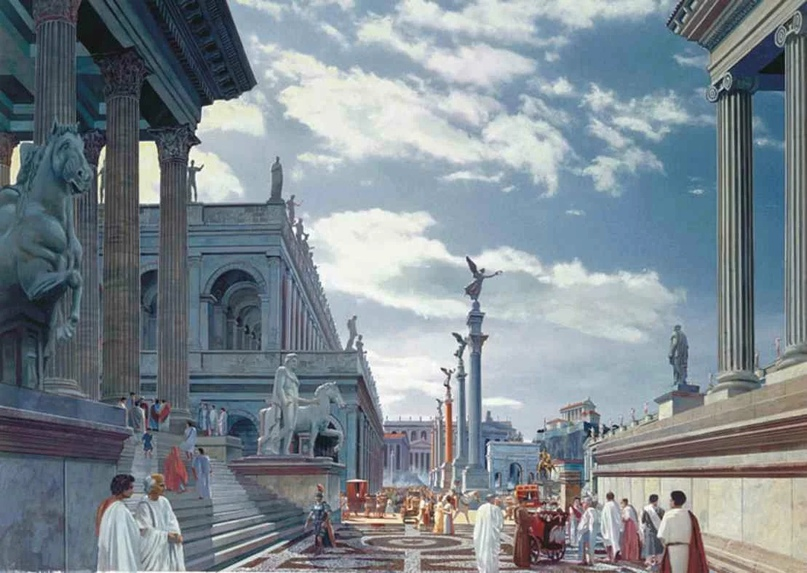
\includegraphics[scale=0.5]{Relig_gambit/1572932193123151938.png}
	\label{fig:gambit4} % Unique label used for referencing the figure in-text
	%\addcontentsline{toc}{figure}{Figure \ref{fig:placeholder}} % Uncomment to add the figure to the table of contents
	
\end{figure}

\textit{«Отношение к религии в Древнем Риме, особенно средне-позднего его периода истории, от Принципата и далее, что обычно и принято знать как "Рим", было похоже на отношение к государственной идеологии в конце СССР. То есть: существуют официальные государственные культы "Гения"(духа) Императора, их надо было формально исполнять, верить в них было необязательно, это был элемент государственной идеологии и "порядка". Вот ты чиновник, значит у тебя должен быть портрет генсека в кабинете, нужно выступать раз в месяц на партсобрании, платить партвзносы, и вот это вот все.Были всякие замшелые верования, типа культа Весты, которые тоже государство рассматривало как "духовные скрепы", но всерьез уже никто не рассматривал.Это все что касается "официальных" религий.Были разнообразные "домашние" верования, все эти Лары, Пенаты, и прочие мелкие "домашние" боги-духи. Это примерно как наши верования в привидений, домовых, леших, "постучи по дереву", "поплюй через плечо" и "посиди на дорожку".И было множество ярких массовых религиозных движений, обычно "иностранных", по которым сходила с ума временами вся Империя. Это аналог каких-нибудь Кашпировских. Все эти культы Изиды, Сераписа, ближневосточные мистерии, и так далее.Одним из них как раз и было сперва христианство.»} (с) Лучше и не скажешь.
\section{Последствия}

Вера стала единой, появилась идентичность, это продлило имперке срок существования примерно на столетие, хотя и имело некоторые неприятные последствия вроде закручивания идеологических гаек или религиозных погромов. Большую часть античного культурного наследия расхуярили не варвары какие-нибудь, а вполне системные религиозные фанатики, в рамках своей борьбы на умы масс. Варвары уже доламывали остатки. Факт - единственная конная статуя дошедшая к нам с античности это Марк Аврелий второго века. Его принимали за Константина Великого (император-христианин, каконизирован), поэтому не трогали. Такие вот дела. Остальное всё сломали, до чего дотянулись. Но, однако, античное наследие - не слишком высокая цена за выживание империи, на самом деле. 

\begin{figure}[h!tb]
	\centering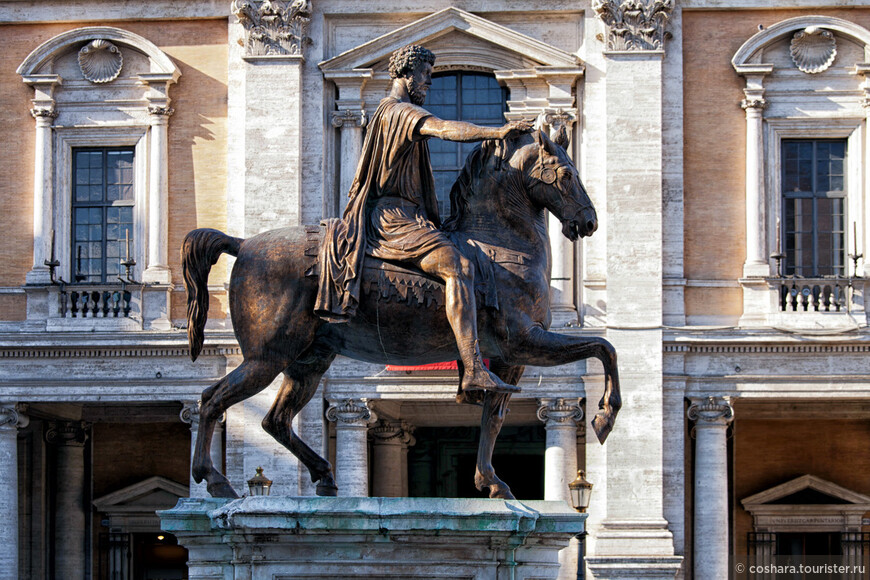
\includegraphics[scale=0.5]{Relig_gambit/157293223814548021.png}
	\label{fig:gambit5} % Unique label used for referencing the figure in-text
	%\addcontentsline{toc}{figure}{Figure \ref{fig:placeholder}} % Uncomment to add the figure to the table of contents
	\caption{	Та самая статуя.	}
\end{figure}
\section{ Гибель Империи}

Имперка всё равно рухнула, как вы помните. Не под страшными внешними ударами, а в силу естественной деградации. Собственные федераты разобрали её куски себе в наследство, напилили варварских королевств и стали жить-поживать. И вот тут религия сделала свой главный ход конём, который отбивает все прошлые и будущие издержки от её существования в нашей объективной реальности. Религия, как я уже говорил, равно идеологии. А идеология - товар экспортный, особенно если у соседей её в принципе не существует в силу общественного устройства. Это страшное идеологическое оружие, которое в прямом смысле переваривает народы без прямой военной оккупации. Когда римляне получили эту свою религиозную дубинку у них как раз закончился жуткий Кризис Третьего Века, в результате которого римская армия перестала существовать, Империя пережила тяжёлый экономический кризис но не пережила кризис управления. Последний вошёл в хроническую стадию, и после этого моменты когда империя хоть чем-то управляла на докризисном уровне, её решения были своевременно и эффективны - можно по пальцам пересчитать. И, одновременно с этим, просрав свою лучшую в мире армию и не способная никакие проблемы решать в реальном времени - имперка возвращается к истокам. Когда я про Раннюю Республику говорил, то отмечал, что в то время римская армия была говном, и поэтому римляне мастерски владели "мягкой силой", политическими многоходовочками, и очень любили решать свои проблемы чужими руками. Тут пришлось вернутся к данной практике, и заняться окультуриванием федератов, где первую скрипку играло именно христианство, в своей экспортной версии. 
\begin{figure}[h!tb]
	\centering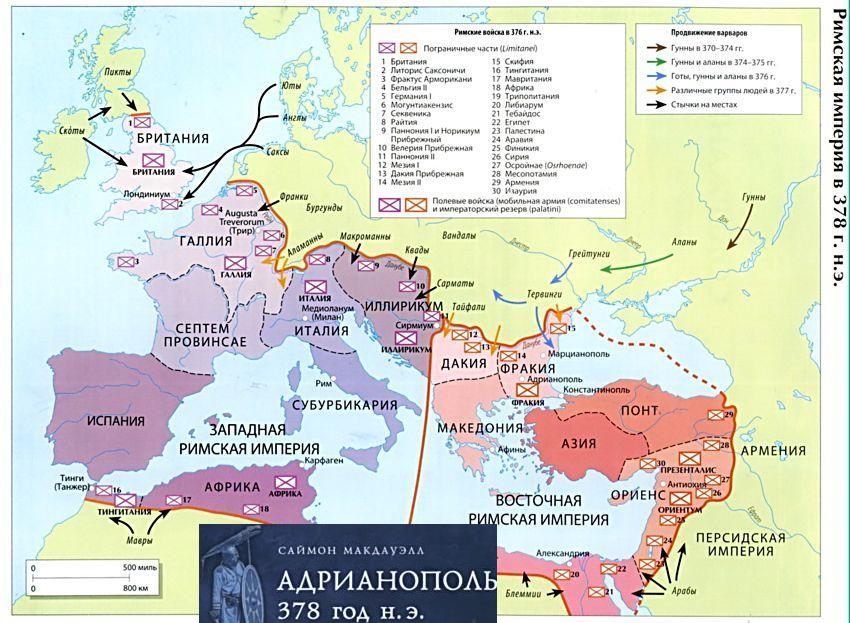
\includegraphics[scale=0.55]{Relig_gambit/1572932315145887007.png}
	\label{fig:gambit6} % Unique label used for referencing the figure in-text
	%\addcontentsline{toc}{figure}{Figure \ref{fig:placeholder}} % Uncomment to add the figure to the table of contents
	\caption{Такие дела. 	}
\end{figure}

\section{Варварские королевства}

Федераты это варвары, да. Они жили себе за Рейном и Дунаем, торговали с Римом, находились под его культурным влиянием, и иногда, канешн, грабили убивали, но глобально - они хотели быть римлянами. Очень хотели. Варварские риксы очень хорошо понимали что вообщет они живут в говне и молятся каким-то корням, и им это было вообще не очень интересно, тем более когда в паре сотен километров развитая цивилизация с дорогами, городами и акведуками. Тоесть там и до Кризиса всё было более-менее хорошо, а после него, когда большую часть этих самых варваров Рим официально берет на службу и начинает платить жалование - стало совсем хорошо. Варварские верхушки принимают христианство практически поголовно, это было одним из условий работы на Рим, а затем и сами Федераты постепенно романизируются и христианизируются. Фактически, когда всё рухнуло, то через Рейн попёрли не какие-то дикари времен Цезаря, а братушки во Христе, которые аккуратно, деликатно входили в права наследования, ничего не ломая и не уничтожая, мягко (ну, для варваров) перехватывая управление. Вот например франки, Франское королевство раскинулось на территории двух римских провинций, но у нас нет свидетельств особо лютой жести. Города существовали, дороги чинили, акведуки работали, ремесленники ремеслили, всё было как раньше. Даже имперские чиновники по большей части остались на местах. Прост сменился слой знати, его заняли франкские варлорды. Ну и монополия на насилие перешла к ним, естественно. При этом когда пришли гунны, реальные варвары, которые всё руинили и жгли, то опиздюливала их на Каталуонских Полях сборная христианских (!) варварских королевств во главе с Аэцием. Которая собралась в основном потому что она христианская, и федераты считали себя прямыми наследниками Империи, без всяких шуток. Соответственно, им было не очень интересно уступать её каким-то унтерам-гуннам. А ещё через пару десятков лет ЗРИ наконец-то закончилась и Одоакр сверг последнего западного римского недоимператора. Затем, чтобы окончательно зафиксировать ситуацию, он собрал императорские реликвии и отослал их в Константинополь, действующему римскому императору, хехе, формально признавая его власть. 

\begin{figure}[h!tb]
	\centering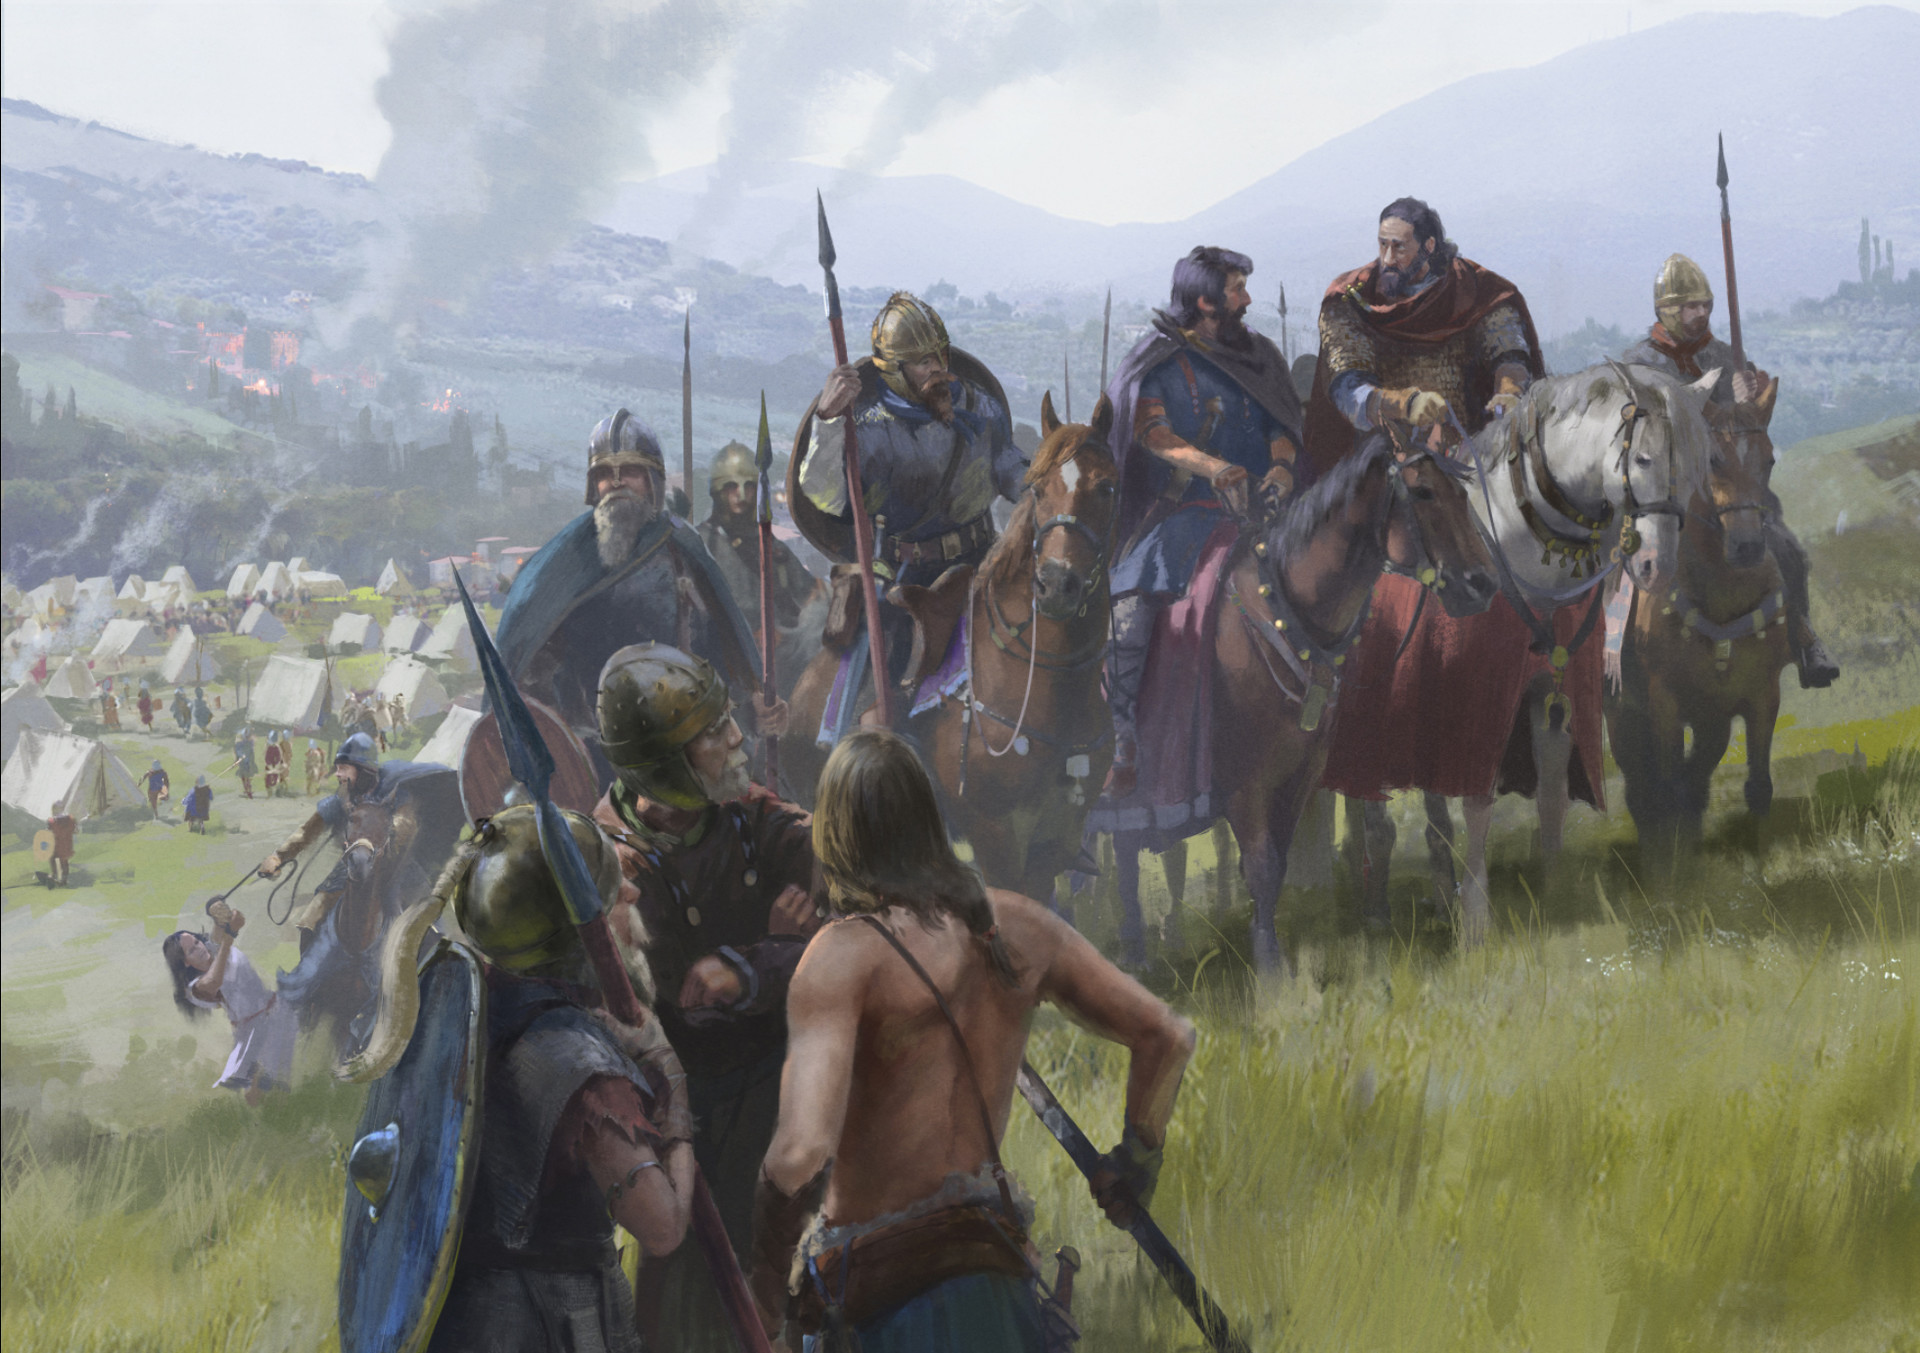
\includegraphics[scale=0.25]{Relig_gambit/157293236414589357.png}
	\label{fig:gambit7} % Unique label used for referencing the figure in-text
	%\addcontentsline{toc}{figure}{Figure \ref{fig:placeholder}} % Uncomment to add the figure to the table of contents
	\caption{Какие-то федераты, скорее всего готы, осматривают свои новые владения. 	}
\end{figure}

\section{Судьба Британии}

Теперь, чтобы не быть голословным, приведём обратный пример. Когда легионы были выведены из Британии, то там в течении нескольких лет случился немножко геноцид. Я серьёзно. Пикты и прочие НЕхристианские унтера полезли с севера и востока, раздавили местное сопротивление и затем уж хуй знает что там творилось, но в этот период у местного населения меняется генокод и следы британских кельтов там с тех пор почти исчезают. Тоесть они вырезали столько мужиков и выебали столько женщин, чтобы нам это отсюда было видно при исследовании останков, лол. Естественно что от городов ничего практически не осталось, огонь цивилизации был потушен и даже обоссан, после чего культурный уровень аборигенов вернулся на доцезарианский - ковыряние палкой-копалкой в жопе, человеческие жертвоприношения и вся подобная хуйня. Британия погрузилась не просто в Тёмные Века, она рухнула в Пиздец Какие Темнющие Века, а цивилизация и государственность были снесены под котлован. Ровно то же самое ждало и континентальных римлян, еслиб они в свое время не подстелили соломки, пару столетий старательно моя своим федератам мозг, превращая их в своих братьев по разуму и во Христе. Более того, у нас есть отличный пример Атиллы, который собрал вокруг себя кучу всяких нецивилизованных варваров, и они, в своём походе на ЗРИ, занимались именно тем, чем и положено заниматься варварам-ортодоксам - жгли, резали и ебали всё что видели перед собой. Христианизация федератов спасла территории бывшей ЗРИ от полного разорения, и ещё лет сто там, на уже бывшей территории бывшей Империи, шли встречные процессы деварваризации варваров и варваризации ромеев, пока всё не зафиксировалось на уровне чуть ниже среднего.
\begin{figure}[h!tb]
	\centering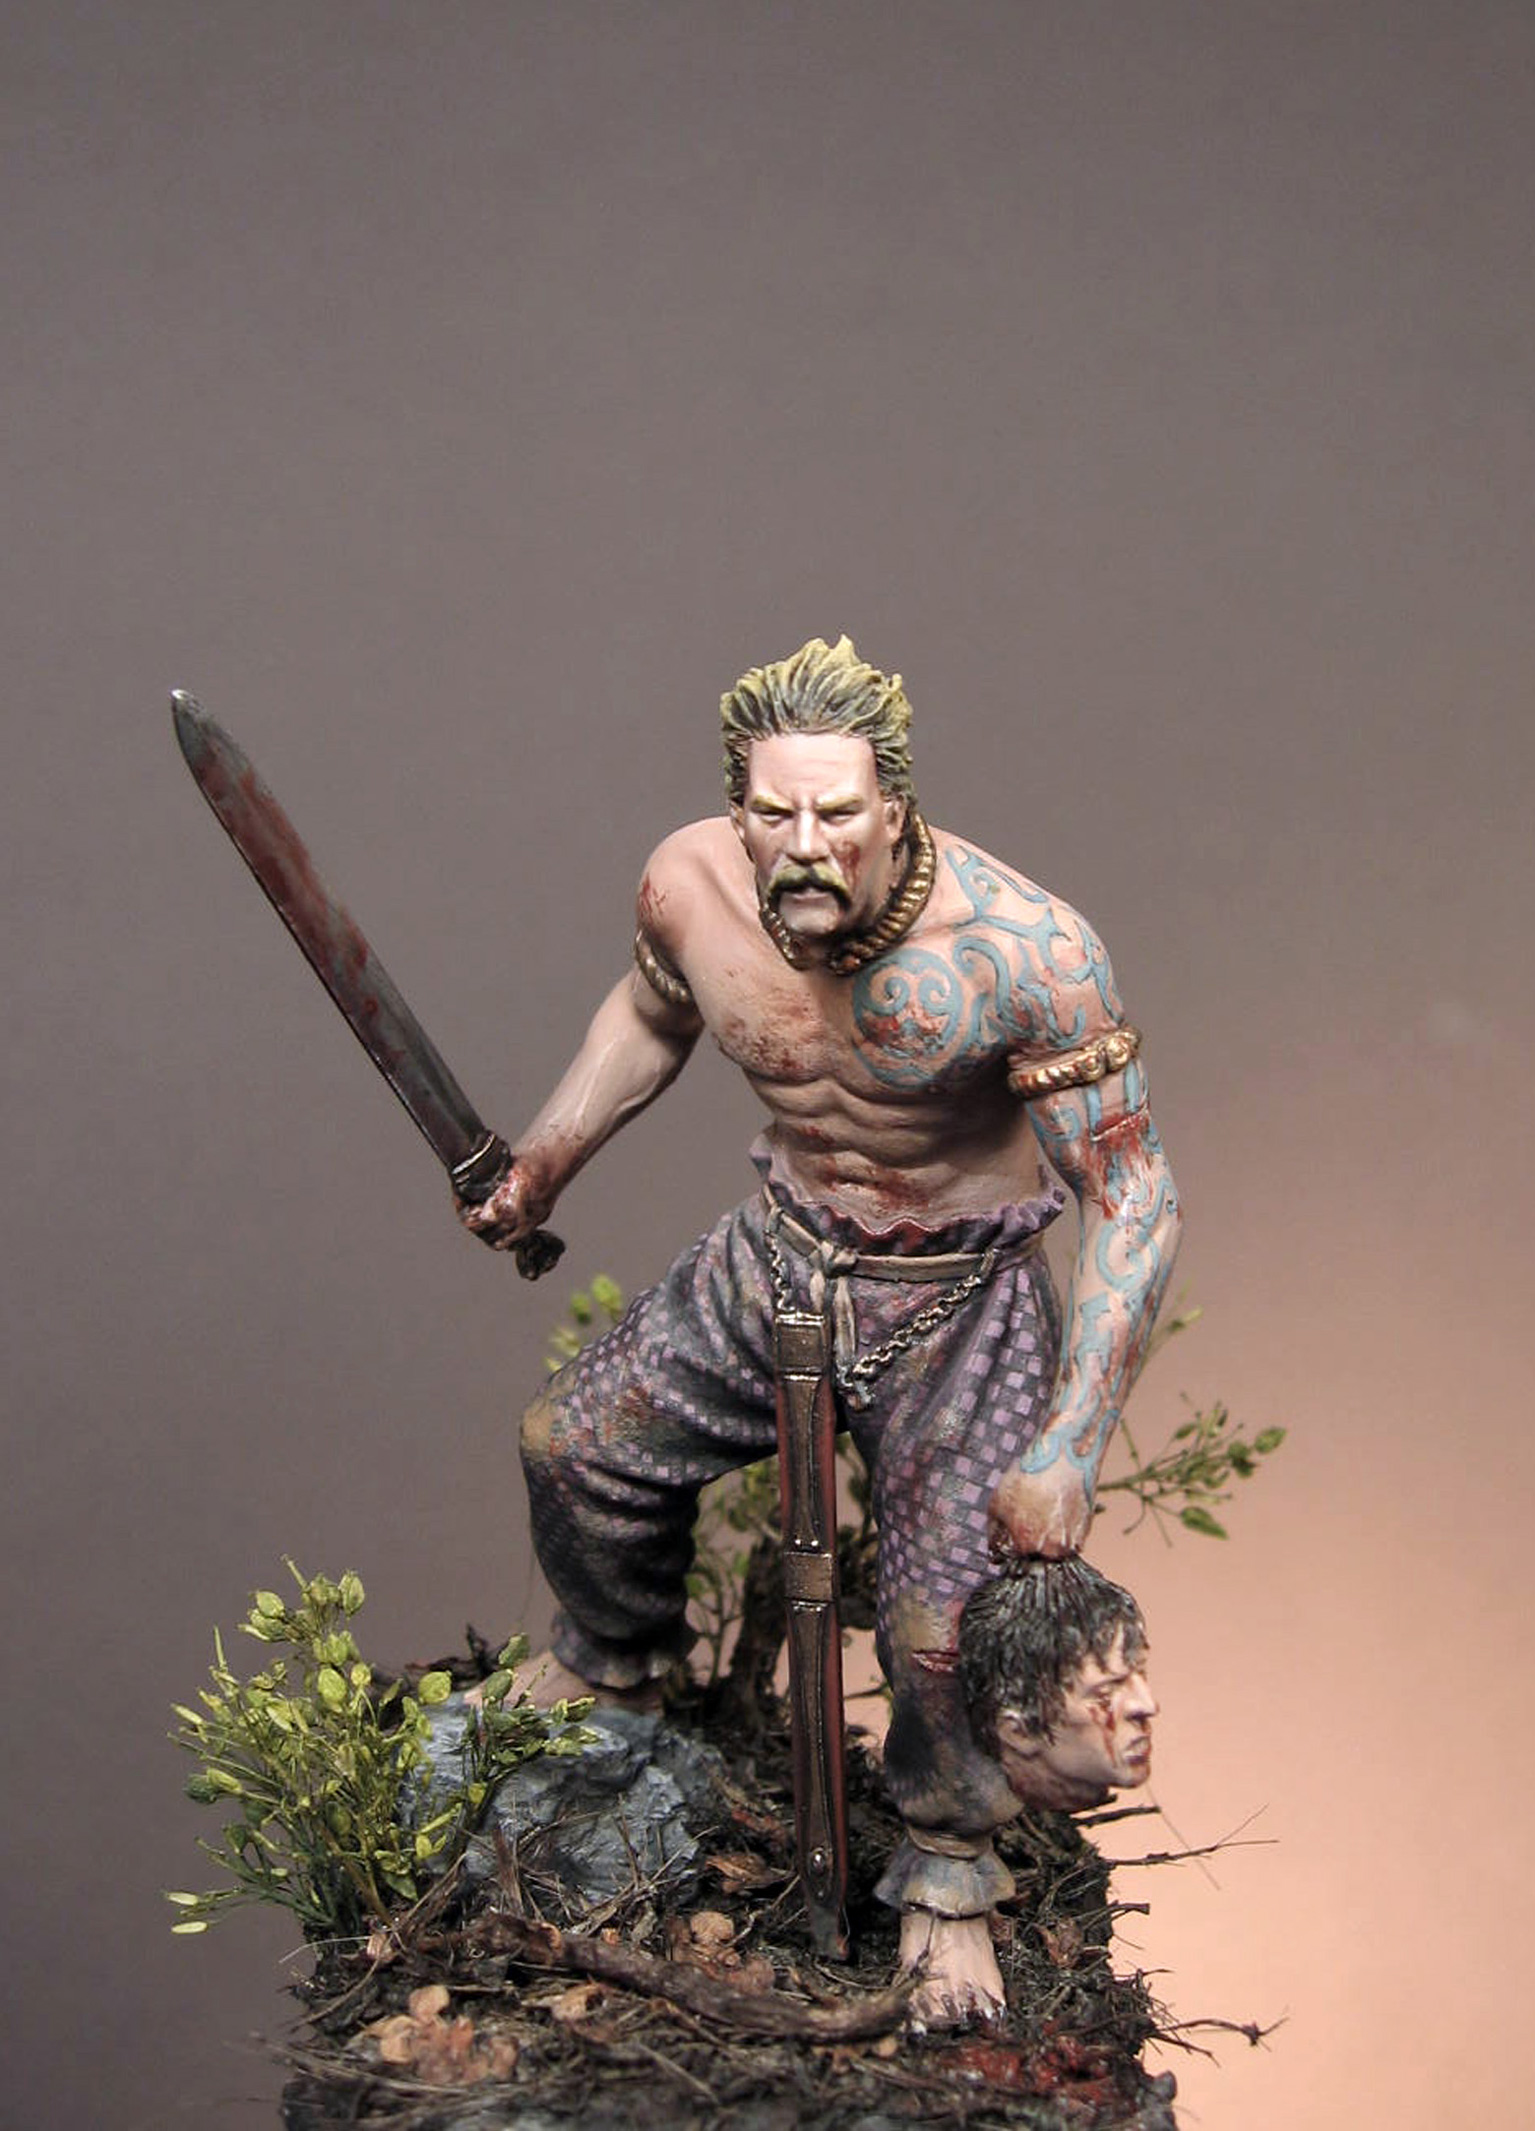
\includegraphics[scale=0.2]{Relig_gambit/1572932401136943899.png}
	\label{fig:gambit8} % Unique label used for referencing the figure in-text
	%\addcontentsline{toc}{figure}{Figure \ref{fig:placeholder}} % Uncomment to add the figure to the table of contents
	\caption{Типичный пикт из палаты мер и весов	}
\end{figure}

\section{Попытка реванша Восточной Римской Империи}

Я вот уверен что данный исход предусматривался римскими стратегами. Сомневаюсь что они именно так всё планировали, но учитывая что имперка по швам трещала не первое столетие, то выпадение отдельных регионов из под контроля Римом было, считай, неизбежностью. А теперь следите за руками. Вот мы в прошлом пункте посмотрели как оно бывает на примере бриттов. Вывел ты легионы на пару лет, потом возвращаешься, а там уже полный пиздец. Вся долгая, кропотливая работа по построению инфраструктуры и отучиванию местного населения подтирать жопу лопухами - коту под хвост, там всех убили и всё разрушили. Заново чтоле ещё лет двести туда ресурсы вливать чтобы опять этих ябучих дикарей делать римлянами? Вот и я думаю что оно никому не интересно. Поэтому план был такой - создаём единое культурное пространство, и всех возможных отжимателей территорий превращаем в себе подобных. Единый язык (латиница, хуле, она и сейчас в основе большей части европейских языков), религия, культура, максимальное приближение к римскому идеалу. Затем повторяем этот процесс лет сто-двести, и вот уже этим мудакам можно и регионы сдавать, не боясь что они там за пару лет всё под котлован сровняют. Более того, еслиб имперка вылезла из кризиса, то она бы с относительной лёгкостью подчинила себе эти относительно цивилизованные народности. Не сложилось с этим делом, но тут нет их вины. Велирисарий через пол века после окончательного падения ЗРИ достаточно легко завоёвывает Африку и часть Испании, а потом ведёт тяжёлую, но успешную войну в Италии, практически восстанавливая Империю в её прежних границах. Потом приходит чума, тяжелейшая война с Парфией, а мусульмане добивают. Крч, с реставрацией как-то не сложилось, в силу внешней коньюктуры, но все условия для этого были в наличии, именно благодаря культурной идентичности. Варварские королевства - часть христианского мира, а в этом мире только одна империя, со столицей в Константинополе. И то что она ебашила формально подчинённых себе королей руками Велирисария - это вполне в рамках этой протофеодальной логики. В общем - пацаны к успеху шли, не подфартило. 
\begin{figure}[h!tb]
	\centering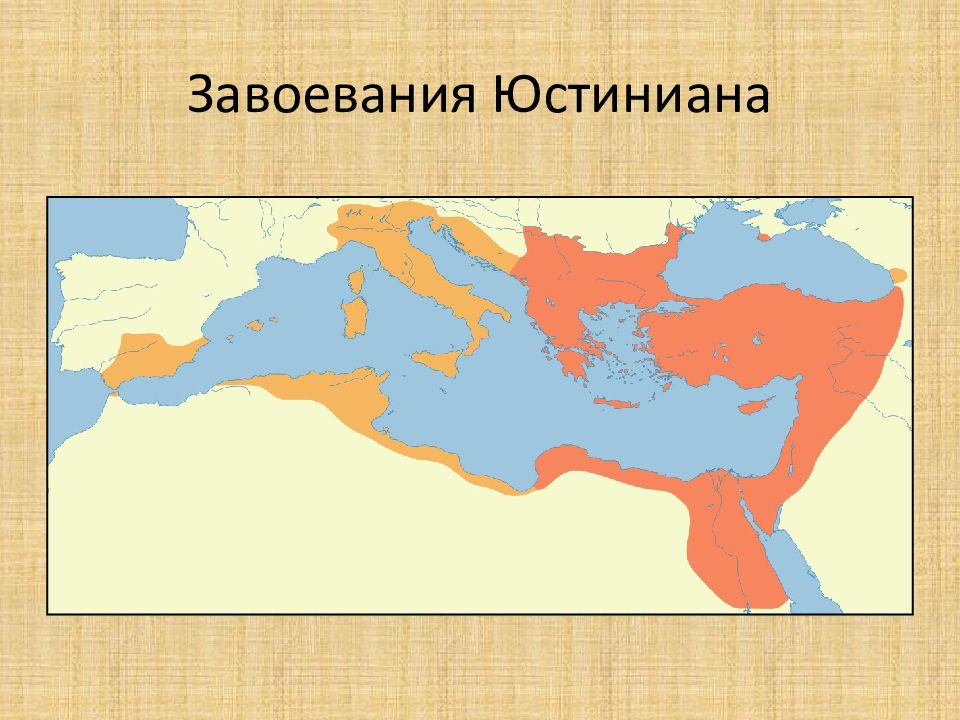
\includegraphics[scale=0.4]{Relig_gambit/15729324551801232.png}
	\label{fig:gambit9} % Unique label used for referencing the figure in-text
	%\addcontentsline{toc}{figure}{Figure \ref{fig:placeholder}} % Uncomment to add the figure to the table of contents
	\caption{Почти, почти шмогла Византия при Юстиниане реставрироваться в прежних границах, но увы. Это у нас 527—565 годы	}
\end{figure}
\begin{figure}[h!tb]
	\centering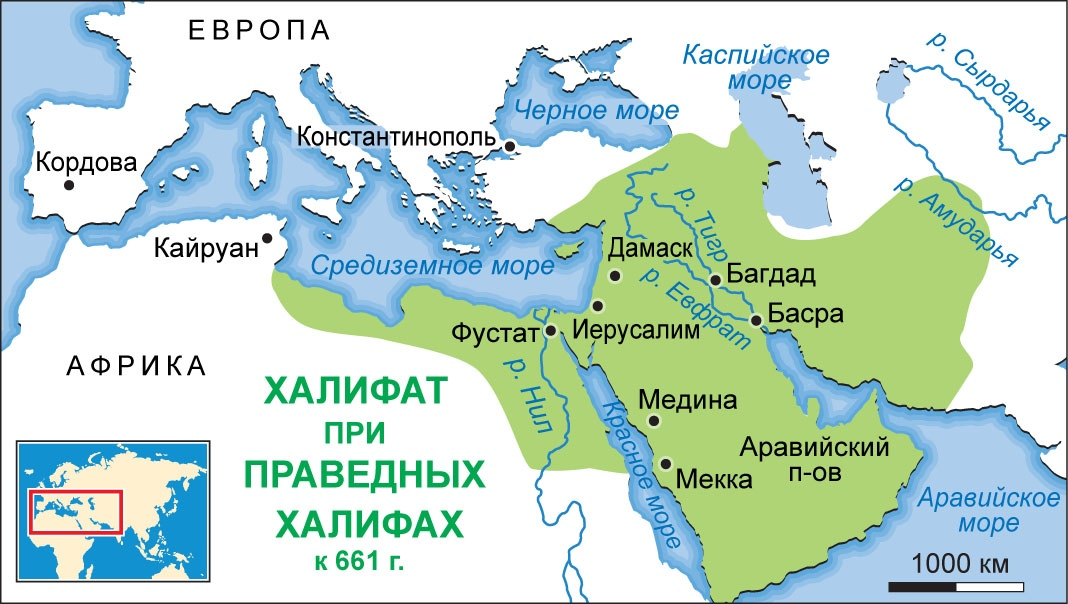
\includegraphics[scale=0.4]{Relig_gambit/1572932481163266824.png}
	\label{fig:gambit10} % Unique label used for referencing the figure in-text
	%\addcontentsline{toc}{figure}{Figure \ref{fig:placeholder}} % Uncomment to add the figure to the table of contents
	\caption{А это спустя всего один век. Арабы поедают 2/3 территории Византии, забивают её в угол и она следующие века только и делает что пытается выжить в этом сложном и тяжелом мире. На этом попытка реставрации Римской Империи прямыми потомками этих самых римлян — заканчиваются.	}
\end{figure}

\section{Темные Века}

Византия из исходника для восстановления Римского Мира превратилась в региональную державу, все силы бросающую на борьбу с расползающимися муслимами, чума перехуярила ~90 миллионов в основном городского населения, наступают Тёмные Века. Века реально Тёмные, и наступают только сейчас, в начале седьмого века. До этого всего лишь отцветала осень античности, всё ещё можно было как-то реанимировать, христианский мир корежило, но он проявлял себя очень жизнестойким помидором. Потом уже всё. Муслимы в Испании, Италия разорена, чума уничтожила остатки античной цивилизации, Византия в дауне. И ситуация выглядит безнадежной. И тут внезапно выясняется что в этом первичном бульоне, где государства погибли, идёт война всех против всех и никто не понимает что происходит, единственная организация сохранившая какой-то контроль над христианским миром в целом - христианская церковь. Данная контора ни с кем не воевала, сопала свои религиозные грядки и пользовалась, в наступившем вакууме, неплохими привилегиями. Главное что у них было это легитимность, которую они могли отгружать варварским королям, и превращать их из каких-то ноунеймов в божьих помазанников, за что и пользовались практически полной неприкосновенностью, хоть и не имели какого-то собственного силового ресурса. Да и муслимы лезли со всех щелей, а против неверных все мы правоверные, как известны. Крч, какие-то глобальные движи в рамках этих Фаллен Штатов могла организовать только церковь, и именно она не дала этому скорее уже не Римскому а Христианскому Миру расползтись по швам. Кроме того, после чумы и войн города как источники знаний и специалистов утратили своё значение, зато очень сильно поднимаются монастыри. Именно там можно было хотяб научится читать и писать, а также какой-то базовый курс знаний получить. Итого, в этот период церковь спасает осколки античного знания, чё осталось после всех прошедших пиздецов, кое-как координирует действия варлордов на местах, придаёт их правлению легитимности. В самый тяжёлый для Европы период, когда можно было реально скатить пол континента в совсем уж ебучее варварство, именно церковь вытаскивает катку. 
\begin{figure}[h!tb]
	\centering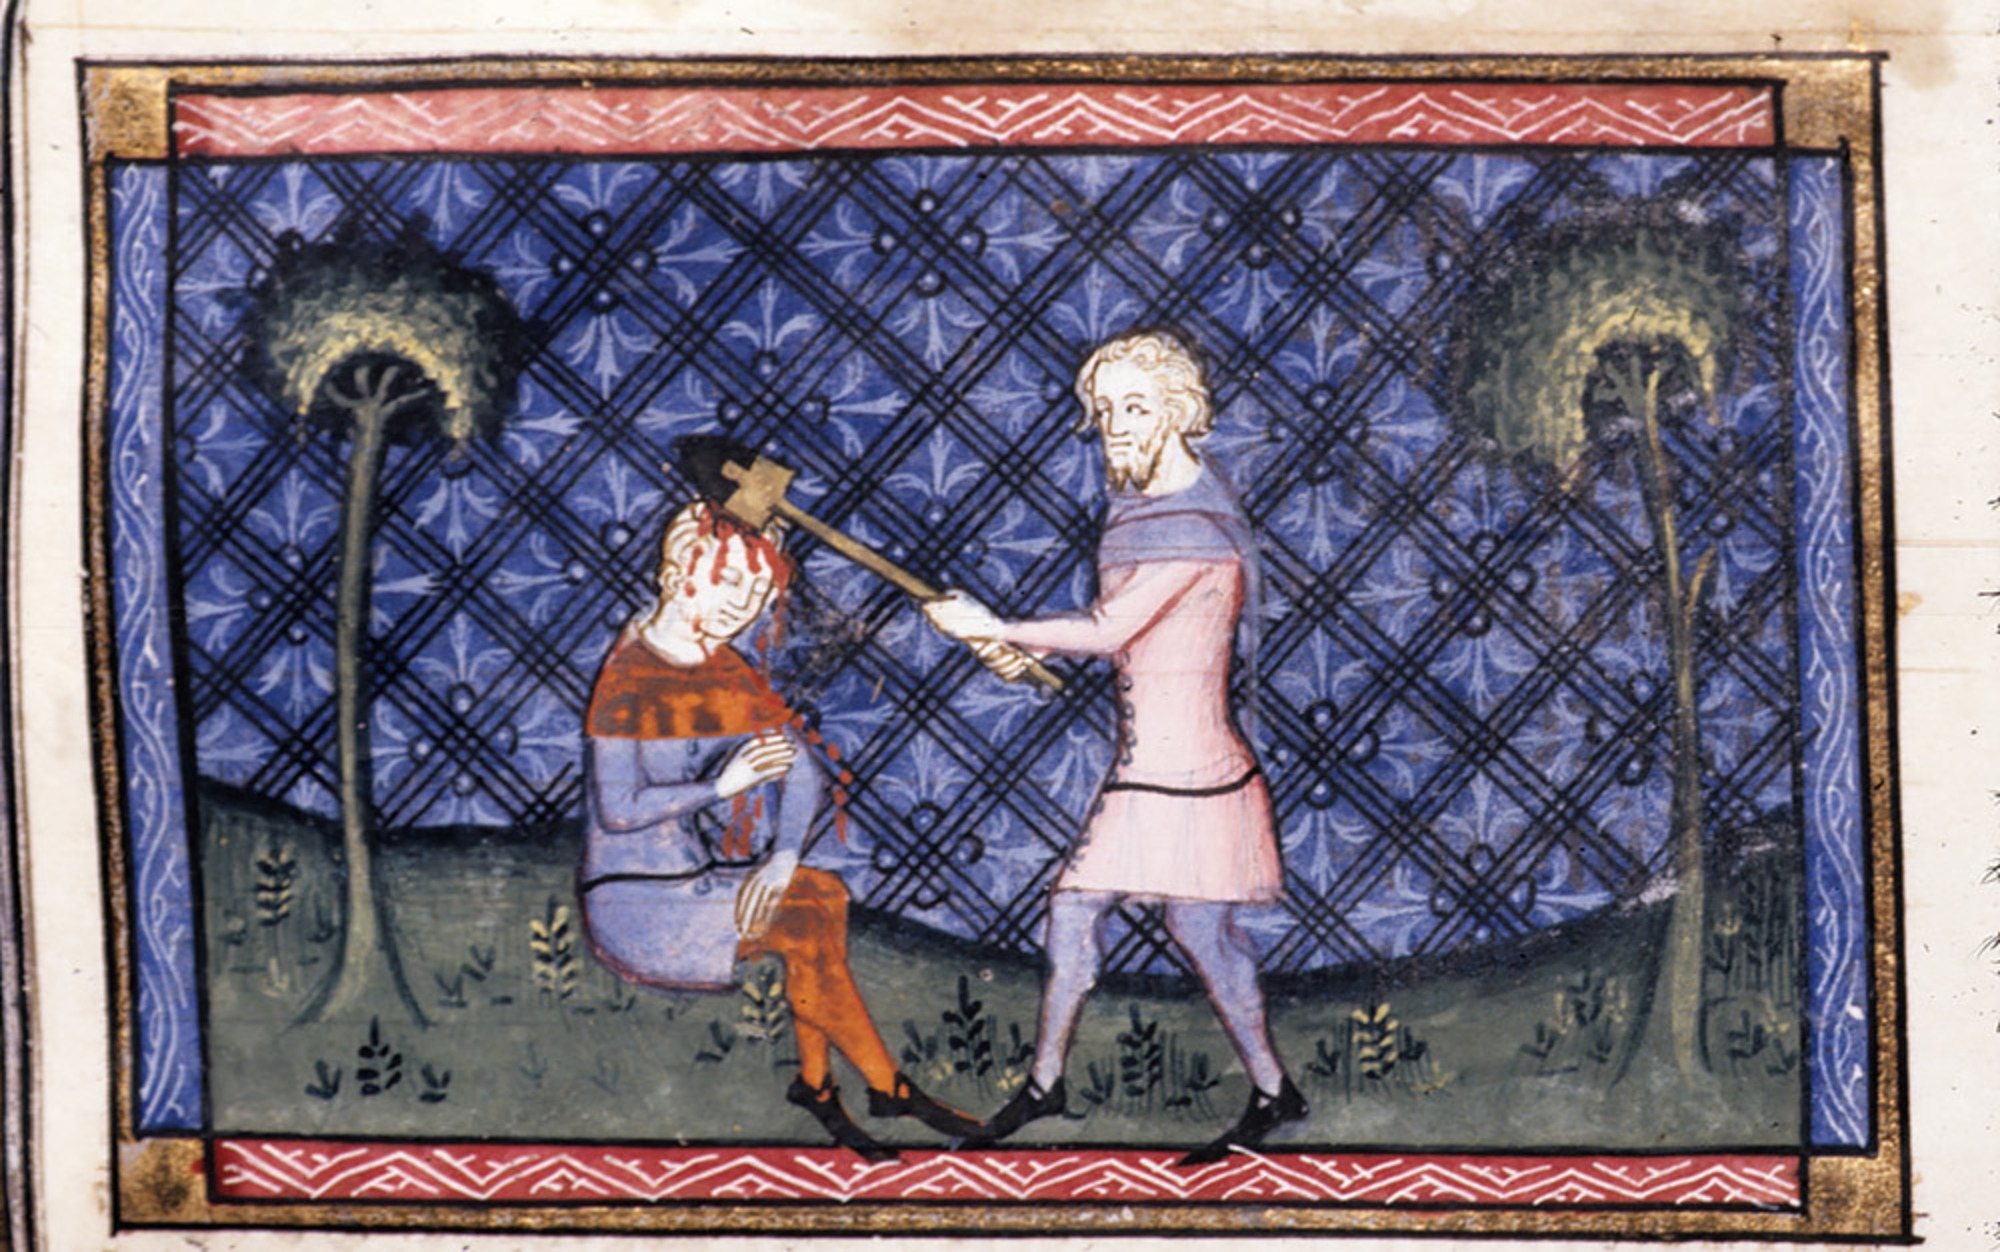
\includegraphics[scale=0.2]{Relig_gambit/1572932526111883618.png}
	\label{fig:gambit11} % Unique label used for referencing the figure in-text
	%\addcontentsline{toc}{figure}{Figure \ref{fig:placeholder}} % Uncomment to add the figure to the table of contents
	\caption{Типичное занятие европейцев в период между падением Рима и воцарением франков, хехе.	}
\end{figure}

\section{Императоры запада}

Затем начинается период франков. Как вы поняли, главное чего добились попы на этот период это сохранили то единое культурное пространство христианского мира, которое римские стратеги ещё второго-третьего веков готовили под себя, чтобы в случае чего суметь сначала схлопнуть а потом быстро развернуть имперку в прежних границах. Западная имперка в итоге сдохла, восточная почти шмогла реставрироваться, но потом тоже почти сдохла, и на пару веков этот процесс остановился. Пока не начали подниматься франки, которые за три поколения всё сделали по красоте. Карл Мартелл объединяет франков и даёт пизды муслимам. Его сын, Пипин Короткий, захватывает все что к полу не приколочено, в том числе и совершает поход в Италию, где дружит с римским патриархом и приобретает, можно сказать, "лицензию на объединение христианского мира крестом и мечом". Ну а сын Пипина, Карл Вёликий, уже разворачивается по полной, объединяя всё до чего руки доходят, коронуется Императором Запада, шлёт нахуй Византию, и закладывает столько охуенных вещей, что я устану их тут перечислять. Это стало возможно потому что союз силы и веры - пиздец какая невывозимая связка в тамошнем христианским мире. 
Фактически, династия Каролингов даже не столько завоевывала, сколько собирала земли, реставрируя ЗРИ. Церковь при ней очень сильно поднимается, закладывается основа для церковного раскола (католики и православные это отсюда), основывается Испанская Марка, которая через лет четыреста закончит Реконкисту и станет Кастилией с Арагоном. На восточных границах создаются буферные зоны чтобы ебаные славяне не набигали. Христианский мир склеивается в одну большую имперку. Очень быстро и очень легко. Чтобы понять что это ненормально почитайте про саксов. Карл с ними воевал тридцать лет, чуть ли не каждый год устраивая походы, и по итогу просто вырезал там всё население под корень, заполонив своими поселенцами. Мне кажется что по уровню превознемогания войны с саксами примерно равны всем остальным войнам. А теперь посмотрите на карту, Саксония это такая блямба на севере, истыканная точками восстаний. Вот тут ключевой момент одиссеи. 
Еслиб церковь не сохранила вкусный и питательный бульончик Христианского Мира, то никакой Карл нихуя бы не смог, вообще. Томушта эти саксонии были бы везде, по всей имперке. И тут бы десяти поколений беспощадно резни не хватило бы, чтобы запилить имперку такого размера. Ничего бы не было, еслиб не церковь, еслиб не христианизация федератов, а в конечном итоге еслиб какой-то седой римский магистрат где нибудь при дворе Диоклетиана не придумал бы весь этот христианский гамбит. Хуй бы мы с вами жили в том мире, в котором мы живём сейчас. Христианская цивилизация погибла бы, и какие-нибудь ебучие гунны дожрали бы остатки, а потом тысячу лет тут был бы мрак, ужас, пиздец и полное, беспросветное говно. 
\begin{figure}[h!tb]
	\centering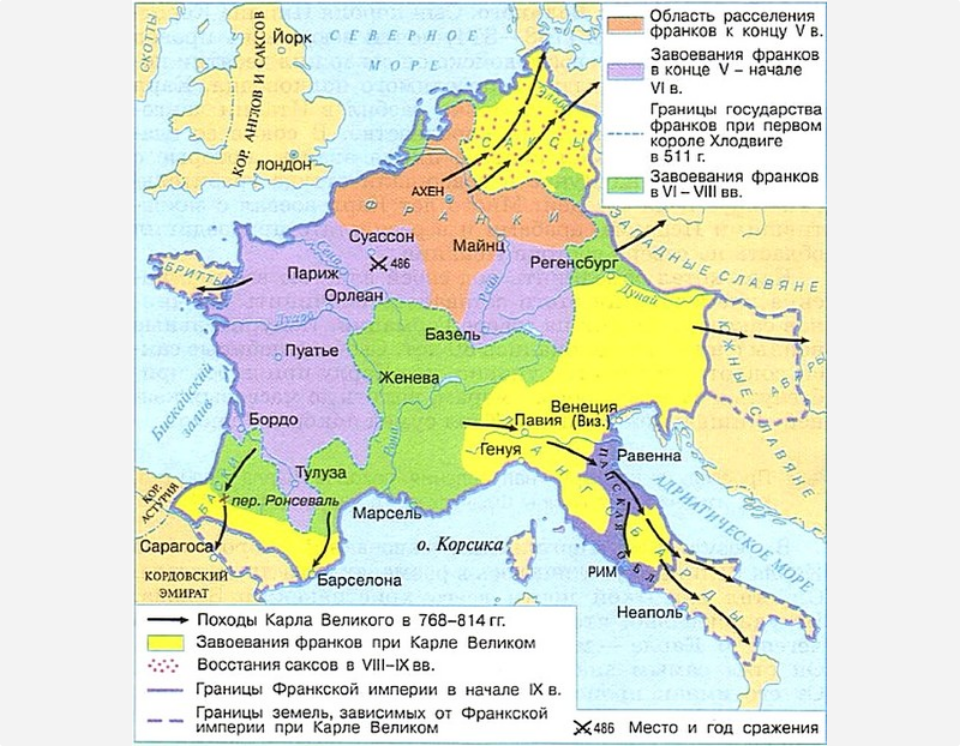
\includegraphics[scale=0.4]{Relig_gambit/1572932602124725131.png}
	\label{fig:gambit12} % Unique label used for referencing the figure in-text
	%\addcontentsline{toc}{figure}{Figure \ref{fig:placeholder}} % Uncomment to add the figure to the table of contents
	\caption{Империя франков при Карле	}
\end{figure}
\begin{figure}[h!tb]
	\centering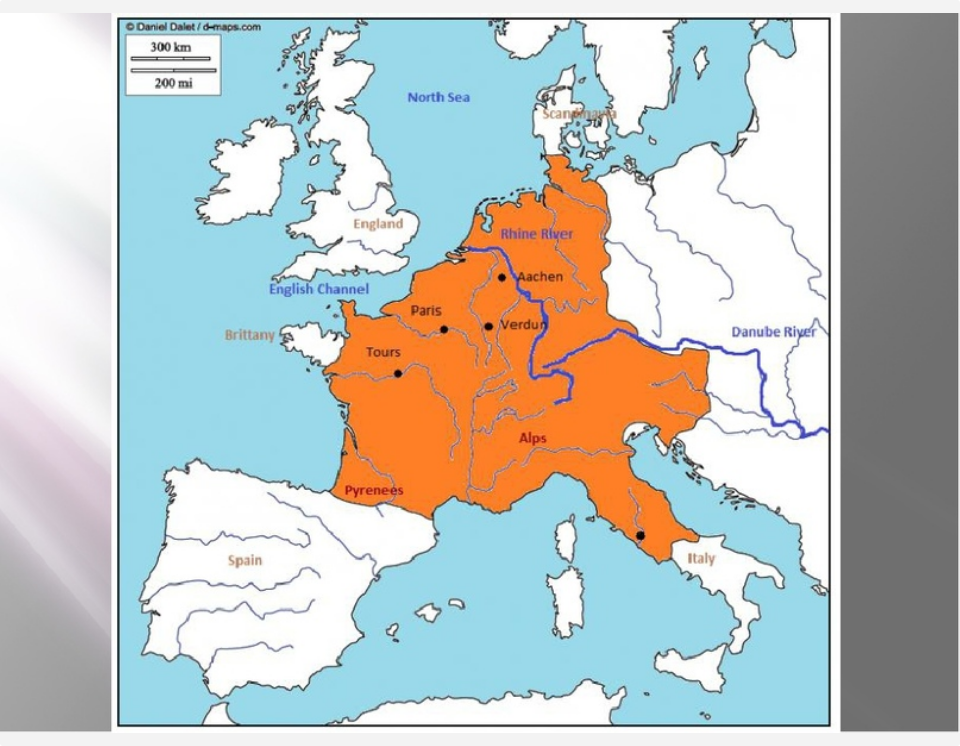
\includegraphics[scale=0.4]{Relig_gambit/1572932634110060550.png}
	\label{fig:gambit13} % Unique label used for referencing the figure in-text
	%\addcontentsline{toc}{figure}{Figure \ref{fig:placeholder}} % Uncomment to add the figure to the table of contents
	\caption{Более понятная карта итогового результата	}
\end{figure}
\begin{figure}[h!tb]
	\centering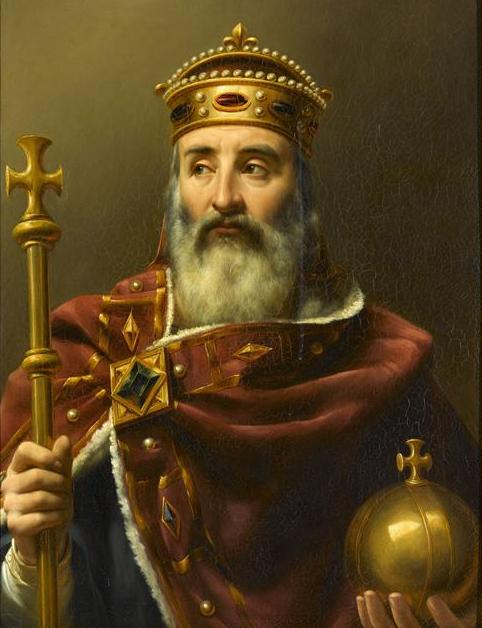
\includegraphics[scale=0.4]{Relig_gambit/1572932654149633403.png}
	\label{fig:gambit14} % Unique label used for referencing the figure in-text
	%\addcontentsline{toc}{figure}{Figure \ref{fig:placeholder}} % Uncomment to add the figure to the table of contents
	\caption{Божею милостью Император Запада собственной персоной, со всякими религиозными штуками в руках. 	}
\end{figure}

\section{Послесловие}

Христианский гамбит сыгран, чего дальше? А дальше имперка Карла уже при его сыне валится на три части, образуя то что потом станет Францией, Италией и СРИ. Но это был именно распад на огромные, жизнеспособные куски, которые просуществуют ещё очень и очень долго. Наступает ранний феодализм, Долгая Зима заканчивается, здравствуй, Средневековье. В этот период церковь продолжает богатеть, но всё ещё прямо не лезет в политику руками, оставаясь неким модератором и моральным авторитетом. Деньги и ресурсы идут на всякие социальные программы, книжное дело ставится на поток, процветают искусства, храмы один другого охуеннее вырастают. У Христианского Мира появляется внешняя политика, пиздить еретиков становится госзаказом, так сказать. Крестовый походы, восточная и северная экспансия, где крестом а где мечом, но обычно в связке. Рождается и обретает силу то чудовище, которое в колониальную эпоху захватит весь мир, всем принесёт слово Господа, цивилизацию, войну и смерть. И вот, как раз на старте Великих Географических Открытий церковь начинает мешать. Мир изменился, усложнился и набрал сил, нянька стала больше не нужна. И вот вам финальный аккорд, так сказать. Церковь, как было сказано выше, является крупнейшим феодалом Европы, самым богатым и мощным. И вот тогда, стартуя Эпоху Возрождения приходит она, Реформация. Суть которой в том, что для перехода от позднего феодализма к нормальным государствам и для образования третьего сословия буржуа нужны, как ни странно, значительные ресурсы. И церкви, за полтора века, пришлось везде на континенте обезжириться, где-то радикально потеряв всё (протестанские страны), где-то поделившись частью накопленный богатств (Франция, СРИ, Италия). Это единовременно вливание в экономику церковных денег подстегнуло колониальную гонку, промышленную революцию, и, в конце концов, дало европейцам завоевать мир. Церковные деньги это, можно сказать, наследство, которое христианский мир получил в год своего совершеннолетия. Последний подарок античной цивилизации своим потомкам.
\begin{figure}[h!tb]
	\centering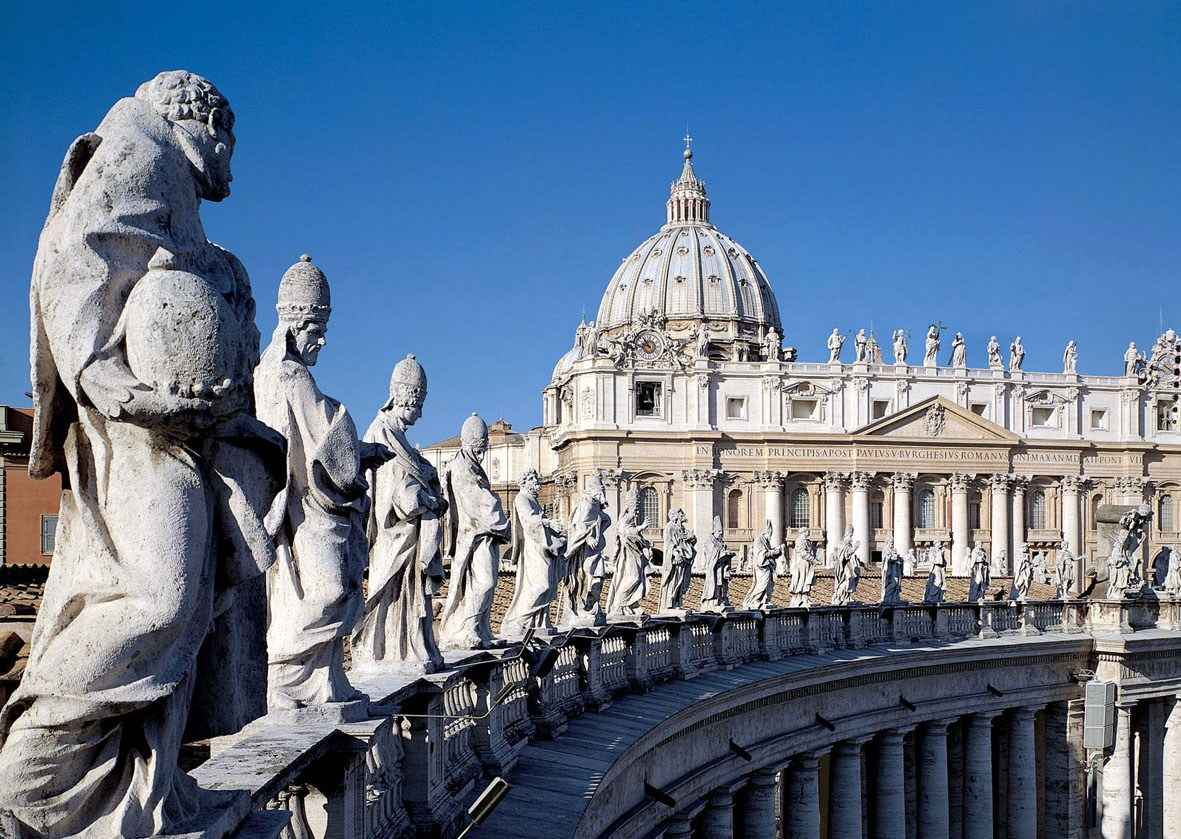
\includegraphics[scale=0.4]{Data/Relig_gambit/157293270319061829.png}
	\label{fig:gambit15} % Unique label used for referencing the figure in-text
	%\addcontentsline{toc}{figure}{Figure \ref{fig:placeholder}} % Uncomment to add the figure to the table of contents
	%	\caption{Типичное занятие европейцев в период между падением Рима и воцарением франков, хехе.	}
\end{figure}
Такие дела. Каждый из десяти тезисов можно разворачивать в статью, канешн, а по послесловие писать отдельный цикл, но я не буду, сказанного более чем достаточно. Однако в комментах могу пояснить за некоторые моменты, задавайте свои вопросы.
